% !TeX spellcheck = en_US
% !TeX encoding = utf8
% !TeX program = xelatex
% !BIB program = bibtex

\documentclass[12pt]{article}
\usepackage[english]{babel}
\usepackage[utf8]{inputenc}
\usepackage{amsmath}
\usepackage{graphicx}
\usepackage[colorinlistoftodos]{todonotes}
\usepackage{enumitem}
% \usepackage{titlesec}
% \usepackage{titletoc}
% \renewcommand*{\thesection}{Problem {\arabic{section}} }
\usepackage[top=1.0cm,bottom=2.4cm,left=2.4cm,right=2.4cm]{geometry} 
% \usepackage{noindent}
\setlength{\parsep}{0em}
\setlength{\parskip}{0em}
\setlength{\parindent}{0em}
% \setlength{\itemsep}{0em}

\title{Linear Optimization -- Homework 1}

\author{Due: Sunday, April  1}

\date{}

\begin{document}
\maketitle

% \begin{abstract}
% 	Enter a short summary here. What topic do you want to investigate and why? What experiment did you perform? What were your main results and conclusion?
% \end{abstract}

\noindent \textbf{Instruction:} Write a report and complete code. Zip and upload them to ftp. \\ 
\begin{itemize}[noitemsep]
	\item Upload:  \\
	- Address: 10.13.72.84 \\ 
	- Username: opt Passwd:  opt18 Port: 21 
	\item Download: \\
	- Address: 10.13.72.84 \\ 
	- Username: opt Passwd:  opt18 	Port: 21
\end{itemize}


{\vspace{1em} } 


\textbf{Problem 1.}
A McCulloch-Pitts (M-P) neuron accepts bipolar input $x_i \in \{-1,1\}$ and gives  $y=\mathrm{sgn} (\sum_{i=1}^{m} w_ix_i + b) $.

Give weights and bias for a M-P neuron with inputs
$x,y,z \in \{-1,1\}$ and whose output is  $z$ if $x = -1$ and $y = 1$, and is $-1$ otherwise.


\vspace{1em}


\textbf{Problem 2.}
The following figure shows the decision regions of four classes. Design a
classifier for these linearly inseparable classes, using a network consists of M-P neurons with
three output units. For class $i$ $(1 \le i \le 3)$, classification requires that $y_i = 1$, with $y_j = -1$ for
$j \ne i$. Class 4 is recognized when $y_i = -1$ for $1 \le i \le 3$. 

\begin{figure}[h]
	\centering
	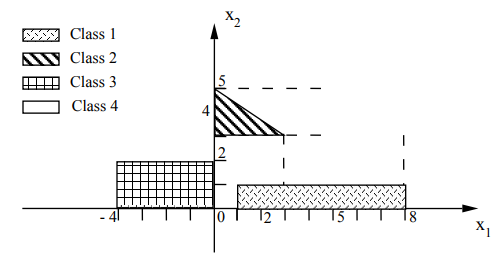
\includegraphics[width=0.7\textwidth]{fig/2018-03-17-14-09-07.png}
	% \caption{\label{fig:frog}This frog was uploaded to writeLaTeX via the project menu.}
\end{figure}



\vspace{1em} 



\textbf{Problem 3.} \label{sec:3}
MLP and BackPropogation:  

\begin{itemize}
	\item Download ``hw2.zip'', The code pass test under Python 2.7.14 and Python 3.6.3. Complete code surrounded by ``TODO'' in ``net.py'' and ``opt.py''. For example, 
	\begin{verbatim}
###########################################################################
# TODO: Implement the affine forward pass. Store the result in out. You   #
# will need to reshape the input into rows.                               #
###########################################################################


###########################################################################
#                             END OF YOUR CODE                            #
###########################################################################
	\end{verbatim}
	\item Run ``python main.py'' and paste the results to  your report. Make sure your code pass gradient check, \textit{i.e.}, relative error between Numerical gradient and analytic gradient is small, \textit{q.g.} smaller than 1e-7. We use centered formula $df(x)/x = [(]f(x+h)-f(x)]/h$ to compute numerical gradient since it has an error on order of $O(h)$ and use relative error as metric. 
	\item Do something extra surrounding the topics in this assignment,  using the code you developed. For example, is there some other interesting question we could have asked? Is there any insightful visualization you can plot? We did not use large cifar10 data. You can select some samples in cifar10 or use the dataset in Problem~4\ref{sec:4} to do real case analysis. 
\end{itemize}


\vspace{1em} 


\textbf{Probelm 4.} \label{sec:4}
Predict House Prices: 
Given 79 explanatory variables describing (almost) every aspect of residential homes, such as the size  and the location of the house, please predict the final price of each home. 

\begin{itemize}
	\item The dataset is cleaned to become simple train/test format. You can try to modify the process of data clean. 
	\item Encourage to do model selection. For example, try lasso regression or humble loss. 
	\item Make sure implement by yourself and do not machine learning related library. You almost implement the algorithm in Problem~3\ref{sec:3}. 
\end{itemize}

\end{document}